%!TEX root = thesis.tex
\hypertarget{functions---encryption}{%
\section{Functions - encryption}\label{functions---encryption}}

The following functions are from `AES\_encrypt.c'
(`Implementation'-chapters). The following chapter is based on \cite{fips197} and the authors own
knowledge/opinions, if not mentioned otherwise.

\hypertarget{key-addition}{%
\subsection{Key Addition}\label{key-addition}}

\hypertarget{description-2}{%
\subsubsection{Description}\label{description-2}}

\begin{figure}
\centering
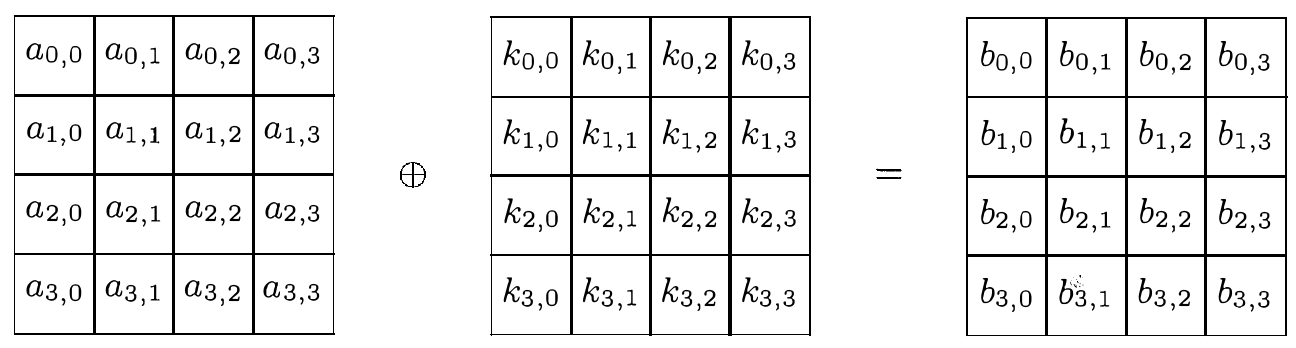
\includegraphics[scale = 0.3]{data/figures/addroundkey.png}
\caption{Addition of the round key to to the state via bitwise XOR. a0,0 xor k0,0 = b0,0 etc.}
\end{figure}

In this transformation a round key is
XORed with the state. The round key array is
derived from the initial cipher key using the key schedule. Containing
16 bytes, each round key is equally long to a block. Since there are N+1
round keys generated (where N is the number of rounds), each round uses
a different round key (ch. 5.1.4).

\hypertarget{implementation-2}{%
\subsubsection{Implementation}\label{implementation-2}}

\begin{lstlisting}
/*
 * Adds the roundkey to a block.
 */
inline void AddRoundKey(uint8_t * restrict bytes,
                        const uint8_t * restrict keys)
{
        for(uint8_t i = 0; i < 16; i++) {
                bytes[i] ^= keys[i];
        }
}
\end{lstlisting}

This function is used to add the current round key to the current block.
It takes a restricted pointer to the first byte of the block the cipher
is currently operating on and a restricted pointer to a constant, which
points to the first byte of the round key, that is supposed to be used
currently. It proceeds to combine each of the sixteen bytes of the block
with a corresponding byte of the round key designated to the current
round using the bitwise XOR. The result is then stored in the block byte
used in the XOR operation, meaning that first byte one of the block will
be XORed with byte one of the round key and then the result will be
stored in place of byte one and so forth for all sixteen bytes.

Since the function is relatively short the `inline'-keyword is used to
save the overhead of an additional function call in trade-off with a
bigger binary.

\hypertarget{shift-rows}{%
\subsection{Shift rows}\label{shift-rows}}

\hypertarget{description-3}{%
\subsubsection{Description}\label{description-3}}

\begin{figure}
\centering
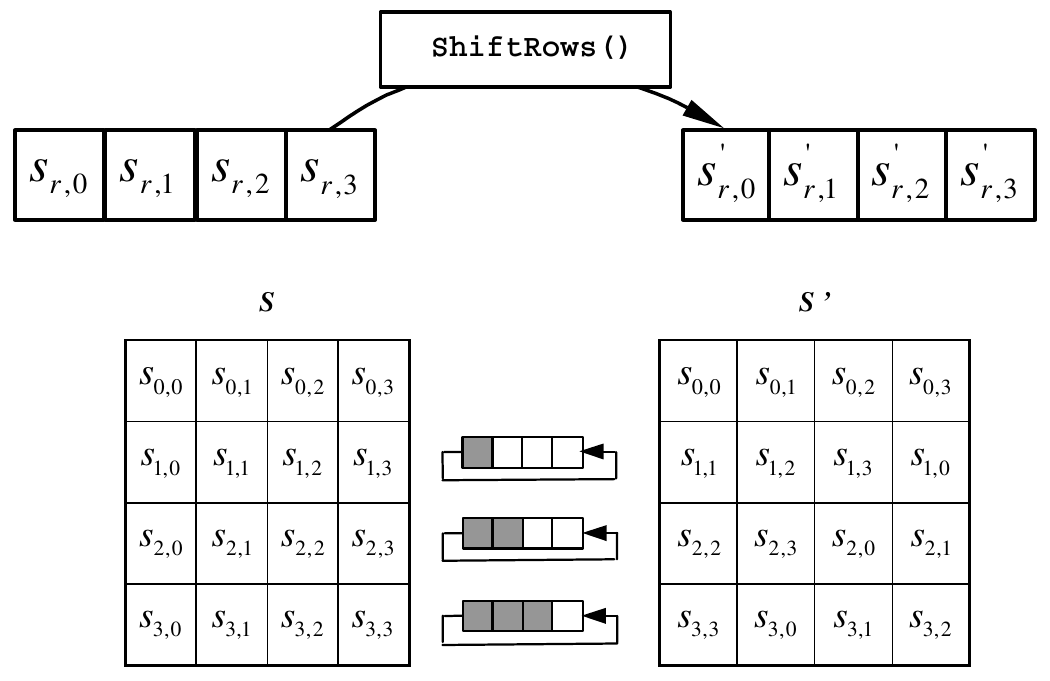
\includegraphics[scale = 0.3]{data/figures/shiftrows.png}
\caption{The ShiftRows-transformation "rotates" the rows of the state (left) by different offsets, resulting in the state on the right}
\end{figure}

\cite[p. 37]{rijndael} states, that this transformation of the state represents a byte transposition, using
cyclical shifts with different offsets. The first row of the 4x4-Matrix
of 16 bytes that constitutes the so called state is not shifted at all,
the second row by one step to the left, the third row uses two steps and
the fourth row three.

According to \cite{rijndael} this transformation step is needed to ensure
optimal diffusion of the state, thus protecting
against differential and linear cryptanalysis. The authors further
elaborate, that in order to archive optimal diffusion all
offsets of the cyclical shifts have to be different.

Since there are multiple possibilities for different offsets and not all
of them provided equal protection, studies of attacks against Rijndael
were analyzed. From the offsets that proved to be the most resistant the
simplest offset was chosen.

\hypertarget{implementation-3}{%
\subsubsection{Implementation}\label{implementation-3}}

\begin{lstlisting}
/*
 * Achieves the AES-ShiftRows by representing it as a series of array-assignments.
 */
void ShiftRows(uint8_t * restrict block, uint8_t * restrict tempblock)
{
        memcpy(tempblock, block, 16 * sizeof(uint8_t));

        block[1] = tempblock[5];
        block[2] = tempblock[10];
        block[3] = tempblock[15];
        block[5] = tempblock[9];
        block[6] = tempblock[14];
        block[7] = tempblock[3];
        block[9] = tempblock[13];
        block[10] = tempblock[2];
        block[11] = tempblock[7];
        block[13] = tempblock[1];
        block[14] = tempblock[6];
        block[15] = tempblock[11];
}
\end{lstlisting}

The function ShiftRows performs the ShiftRows-transformation on the
state. It takes a restricted pointer to the first byte of the block the
cipher is currently operating on and a restricted pointer to a temporary
block. First the content of the block is copied into the array the
tempblock-pointer is marking. After that the row shifts are represented
by assigning the bytes into their positions in the block after the
shifts from the tempblock,

\hypertarget{mix-columns}{%
\subsection{Mix columns}\label{mix-columns}}

\hypertarget{description-4}{%
\subsubsection{Description}\label{description-4}}

The MixColumns-transformation, a so-called bricklayer permutation, had to fulfill
\cite[p.39]{rijndael} multiple design criteria deemed as important by the authors:

\begin{enumerate}
\def\labelenumi{\arabic{enumi}.}

\item
  \emph{The bricklayer transformation is supposed to operate on columns
  containing 4 bytes.} This aspect is supposed to aid with the optimal
  implementation of lookup tables on 32-bit architectures, thus
  ensuring a speedy computation of the transformation.
\item
  \emph{The operation should be linear over GF(2)}, meaning the Galois
  field of the two elements 0 and 1. This property aides the authors in
  their so-called `Wide Trail Strategy' (p.126) which is supposed to
  protect against differential and linear cryptanalysis.
\item
  \emph{The diffusion achieved by this transformation is supposed to
  have ``relevant'' power.} The third property is again supposed to
  support the `Wide Tail Strategy'.
\item
  \emph{The authors put emphasis on the performance of this step on 8-bit
  CPUs.} They deemed this necessary, as they feared that the MixColumns
  transformation would be ``the only step that good performance on 8-bit
  processors is not trivial to obtain for.''(p.39)
\end{enumerate}


\begin{figure}
\centering
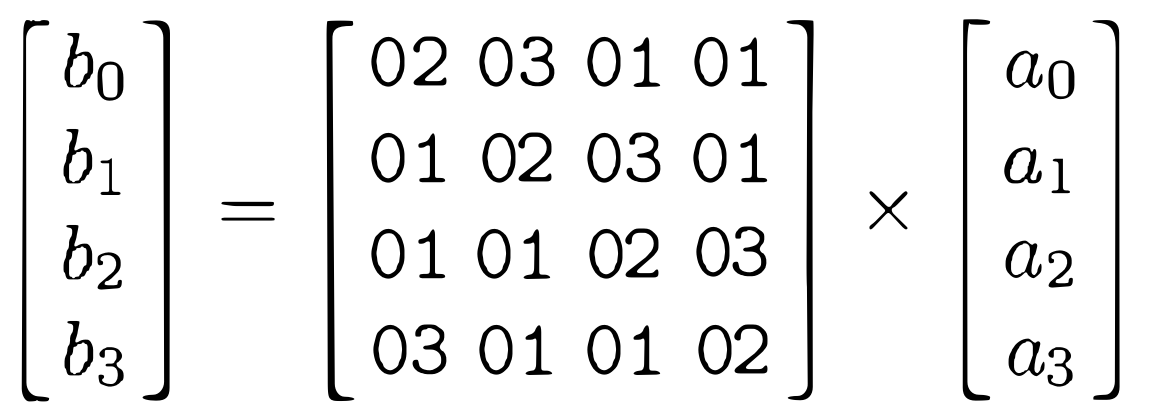
\includegraphics[scale = 0.2]{data/figures/mixcolumn.png}
\caption{The MixColumns-transformation, represented as matrix multiplication.}
\label{fig:mixcolumn}
\end{figure}

The transformation itself partitions the
state-matrix into four columns. Each of those columns is transformed
independently from the other three. A single column acts as a polynomial
over $GF(2^{8})$, which is multiplied modulo $x^4 + 1$ with a fixed polynomial. In
order to meet the aforementioned criteria regarding performance,
diffusion and to fulfill the additional condition of creating an
invertible transformation (in regards to encryption) the authors were
forced to impose conditions on the fixed polynomials \cite[p. 39]{rijndael}. For
example, performance was archived by using only simple values for the
coefficients of the fixed polynomial. The fixed polynomial c(x) Daemen
and Rijmen settled on is $c(x) = 03 * x^3 + 01 * x^2 + 01 * x + 02$. They
state, that since c(x) and the aforementioned modulo $x^4+1$ are coprime
the calculation is invertible. The matrix-multiplication, which is seen
in \ref{fig:mixcolumn}, is a representation of the modular multiplication with a
fixed polynomial.

158 - 88 4.1.1.

\hypertarget{implementation-4}{%
\subsubsection{Implementation}\label{implementation-4}}

\begin{lstlisting}
/*
 * Achieves the AES-MixColumns by representing each result byte as a series of
 * table-lookups XORed with each other.
 */
void MixColumns(uint8_t * restrict block, uint8_t * restrict tempblock,
                const uint8_t (* restrict gal_mult_lookup)[256])
{
        memcpy(tempblock, block, 16 * sizeof(uint8_t));

        for(uint8_t i = 0; i < 16; i += 4) {

                block[i] = gal_mult_lookup[1][tempblock[i]] ^
                        gal_mult_lookup[2][tempblock[i+1]] ^
                        gal_mult_lookup[0][tempblock[i+2]] ^
                        gal_mult_lookup[0][tempblock[i+3]];

                block[i+1] = gal_mult_lookup[0][tempblock[i]] ^
                        gal_mult_lookup[1][tempblock[i+1]] ^
                        gal_mult_lookup[2][tempblock[i+2]] ^
                        gal_mult_lookup[0][tempblock[i+3]];

                block[i+2] = gal_mult_lookup[0][tempblock[i]] ^
                        gal_mult_lookup[0][tempblock[i+1]] ^
                        gal_mult_lookup[1][tempblock[i+2]] ^
                        gal_mult_lookup[2][tempblock[i+3]];

                block[i+3] = gal_mult_lookup[2][tempblock[i]] ^
                        gal_mult_lookup[0][tempblock[i+1]] ^
                        gal_mult_lookup[0][tempblock[i+2]] ^
                        gal_mult_lookup[1][tempblock[i+3]];
        }
}
\end{lstlisting}

The function MixColumns takes multiple arguments. First it takes a
restricted pointer to the first byte of the block the cipher is
currently operating on, followed by a restricted pointer to a temporary
block and lastly the function gets a restricted pointer to the constant,
multi-dimensional GFMLT. MixColumns starts by copying the current state
from `block' into `tempblock'. After that it iterates through every row
by processing 4 consecutive bytes at a time, before it moves to the
following for consecutive bytes of `block'. Each Byte in `block' becomes
the result of four Galois field multiplications combined through the
bitwise XOR-operation, which represents the Galois field addition. The
multiplications are implemented as lookups in the GFMLT and combine the
coefficients of the fixed polynomial c(x) with the bytes of the current
row. After processing all four rows and returning, MixColumns has
written the results of this transformation in place of the current block
being processed.

\hypertarget{substitute-bytes}{%
\subsection{Substitute bytes}\label{substitute-bytes}}

\hypertarget{description-5}{%
\subsubsection{Description}\label{description-5}}

\begin{figure}
\centering
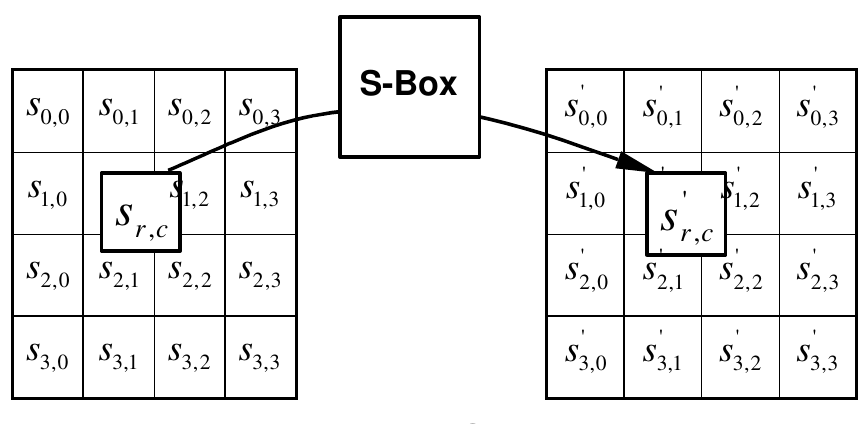
\includegraphics[scale = 0.3]{data/figures/subbytes.png}
\caption{SubBytes applies the S-box substitution to every byte of the
state}
\end{figure}

Being the only non linear transformation, SubBytes is labeled a
bricklayer permutation by \cite[p. 34]{rijndael} that applies byte substitution to
each byte of the state. This substitution is facilitated through the
AES S-box. AES uses
only this one S-box, although the authors mention, that Rijndael ``could
as easily be defined with different S-boxes for every byte.'' (p.35).
They decided against it, because one key criteria during the
development process for them was simplicity (ch. 5.2). Rijmen and
Daemen argue, that simplicity is an important contributor towards a
correct implementation, that it helps to get more people to review it,
since it is easier than reviewing more complex software and that it may
aide the notion it is easier to attack, thus motivating more of such
attacks. They further elaborate that the latter two points contribute to
the cryptographic credibility of the algorithm, especially if out of
many tries no successful attack can be mounted. Furthermore simplicity as
a design criterion was used to balance the security with the factors
efficiency and versatility. This simplicity was partially archived by
designing the algorithm following the principle of what they call
``symmetry''. Their tenet of symmetry within the round transformation
(ch. 5.3.2) " implies that it treats all bits of the state in a similar
way." (p. 66). They explain that this imposes some restrictions, amongst
others the requirement to use only one S-box for the whole state in their
non-linear step. Symmetry across all rounds (ch. 5.31.) dictates that
all rounds have to be identical. This keeps the specification and
implementation short, since only one round has to be described/expressed
in code. This terseness in definition is also of benefit for hardware
implementations, since there has to be only one circuit designed to
implement all rounds, instead of one circuit per round. The other consequence is,
that only one S-box can be used for all rounds.

\hypertarget{implementation-4}{%
\subsubsection{Implementation}\label{implementation-4}}

\begin{lstlisting}
/*
 * Substitutes all bytes in a block with bytes from a sbox.
 */
inline void SubBytes(uint8_t * restrict bytes, const uint8_t * restrict sbox)
{
        for(uint8_t i = 0; i < 16; i++) {
                bytes[i] = sbox[bytes[i]];
        }

}
\end{lstlisting}

The SubBytes-implementation is pretty straightforward. The function
receives two restricted pointers, one called `bytes', pointing to the
first byte of the current state, and one pointer to a constant array,
which contains the S-box to be used. The function now iterates through
`bytes', assigning every element from that array a new value by
accessing the element of the `sbox'-array, which corresponds to the
value in the current `bytes' element.

\hypertarget{full-block-encryption}{%
\subsection{Full block encryption}\label{full-block-encryption}}

\hypertarget{description-6}{%
\subsubsection{Description}\label{description-6}}

To encrypt one block of AES the whole cipher with all rounds has to be
executed. One round consists of four steps, which represent the four
transformation employed in the encryption algorithm. Those transformations are (in that order) SubBytes, ShiftRows, MixColumns and AddRoundKey.
If N is the number of rounds specified by the encryption standard then
the algorithm will execute N-1 * r, while the Nth round omits the
MixColumns step, but is otherwise identical. Before the first round one
additional AddRoundKey is performed on the state. \cite[ch. 5.1]{fips197}

\hypertarget{implementation-5}{%
\subsubsection{Implementation}\label{implementation-5}}

\begin{lstlisting}
void encryptBlock(uint8_t * restrict block, uint8_t * restrict tempblock,
                  const uint8_t * restrict keys, const uint8_t rounds,
                  const uint8_t * restrict sbox,
                  const uint8_t (* restrict gal_mult_lookup)[256])
{
        uint8_t ikeys = 0;
        AddRoundKey(block, keys);
        ikeys += 16;

        for(uint8_t i = 0; i < rounds - 1; i++) {
                SubBytes(block, sbox);
                ShiftRows(block, tempblock);
                MixColumns(block, tempblock, gal_mult_lookup);
                AddRoundKey(block, &keys[ikeys]);
                ikeys += 16;
        }

        SubBytes(block, sbox);
        ShiftRows(block, tempblock);
        AddRoundKey(block, &keys[ikeys]);
}
\end{lstlisting}

The present implementation of the Cipher takes multiple arguments. Like
in all other functions a restricted pointer to the first element in the
state array is provided. The second argument is a restricted pointer to
another byte array of length sixteen, that can be used to store temporary
values. The third argument is a restricted pointer to a constant
byte array, which contains the roundkeys. The next argument is a constant
byte denoting the number of rounds for the algorithm. It is passed to
provide future extensibility in case different key lengths are used and
thus different round numbers are needed, since this number depends on
the key length. The fifth argument is a restricted pointer to a constant
array containing the S-box values. The last argument is a restricted
pointer to a constant, multidimensional array containing the GLFMLT.

The function begins by allocating an unsigned byte on the stack and
assigning it the value of zero. This variable keeps track of the first
byte of the next key that is to be used in the function AddRoundKey,
thus has to be incremented by 16 after every call to the
AddRoundKey-function. The name is derived from ``\textbf{i}ndex of the
round\textbf{keys}''. Next the AddRoundKey-function is called with the
pointer to the current state and a pointer to the first round-key, which
is followed by the first increase of the `ikeys'-variable. Now the
rounds are executed in a for-loop, that counts from zero to the number
of rounds minus one. Every round consists of the following steps:
SubBytes is called with a pointer to the current state and a pointer to
the sbox, followed by a call of ShiftRows with a pointer to the current
state and the tempblock, then a call of MixColumns with pointers to the
current state, the temporary block and the GFMLT. Now comes a call to
AddRoundKey with a pointer to the current state and the memory address
`keys' would point towards, if it was increased by the amount stored in
`ikeys'. The latter passes on the starting address of the bytearray of
the next round key to be used by AddRoundKey. The last part of each
round is the increase of the `ikeys'-counter. After exiting the loop the
function executes one more round without the call to MixColumns and the
increase of the `ikeys'-counter variable and then it returns.

\hypertarget{encryption-of-multiple-consecutive-blocks}{%
\subsection{Encryption of multiple consecutive
blocks}\label{encryption-of-multiple-consecutive-blocks}}

\hypertarget{description-7}{%
\subsubsection{Description}\label{description-7}}

Although not explicitly required in context of this work, the present
implementation contains the possibility to encrypt multiple consecutive
blocks. With that it enables encryption of for example messages larger
than sixteen bytes or even files.

\cite[ch. 5.1.1]{paar} describes
encryption schemes like found in the present implementation the simplest
block cipher modes of operation, called `Electronic Codebook Mode' (ECB).
Every cipher block is generated by simply encrypting the plaintext with
the round keys and appending the encrypted blocks. The first advantage
of this method is that no synchronization between the en- and decrypting
party is necessary, since each block can be processed independently of
each other. Bit errors do not propagate through the whole ciphertext but
are confined to the block they occurred in. The implementation has also
the potential to become very fast, thanks to the possibility of
processing different blocks on different cores, thus enabling
parallelisation of en- and decryption.

The weaknesses of this mode
should not be underestimated though. Due to the fact that every block is
encrypted with the same key, the same plaintexts will generate the same
outputs. If the ciphertext is examined at a block level this is not of
greater significance, since AES guarantees that each encrypted block is
indistinguishable from randomly generated bytes. But if the plaintext as
a whole gets analyzed, patterns may emerge. Those patterns leak
information about what parts of the plaintext contain the same 128-bit
sequence, because those parts also share a bit sequence in
the corresponding ciphertext. Furthermore, a third party watching an
exchange encrypted in ECB can tell, when the same
message is send twice, or if the header of different messages is the
same, for example if each message was using the same salutation. \cite{paar}
demonstrates two attack avenues, that are a direct result of ECB. The
first one exploits the ECB-encrypted communication channel between two
banks. Here the attacker A just needs to open one account on both banks
and review the communication channel for patterns from test transactions
he is sending between the two accounts. If the banks do not rotate keys
A will soon know which encrypted blocks belong to his account number and
which block denote the recieving account in such a test message. After learning that they can
exchange all blocks they know as reserved for the number of the
receiving account with the blocks for their own account number and
divert all transactions between the two banks to A's account. The other
attack avenue is the emergence of patterns visible to the naked eye. For
this example we created an image in the bitmap format(\ref{fig:aespng}). This
image was encrypted with a modified variant of the present
implementations file encryption mode \footnote{Encrypted with the following settings for key generation: key = "passwort", iterations = 20, salt = "aeskurs"}. The modification (inserted just
before the while-loop) ensures that the header of the .bmp-file is
preserved and not corrupted by the encryption. It reads the first 55
bytes (since the header is 54 bytes long
(https://www.daubnet.com/en/file-format-bmp)) and writes them to the
encrypted file without encrypting them. After that, the rest of \ref{fig:aespng}
is read, encrypted and appended. The result \ref{fig:aesecbpng}, albeit encrypted
with an algorithm considered secure, shows a clear and readable pattern.
For comparison we used the `pyaes'-library to encrypt the image in the
same way with the same key\footnote{Encrypted with the following settings for key generation: key = "passwort", iterations = 20, salt = "aeskurs"} and preservation method of the header, but
applied the Counter Mode of Operation. The result, displayed in \ref{figaesctrpng}, demonstrates, that any visible pattern resulting from
ECB-encryption disappears with the right Block Cipher Mode of Operation.
\cite[ch. 5.1.5]{paar} describes how the Counter Mode is an example of block
cipher modes of operation that avoids such patterns. First an
initialization vector IV gets chosen. This ensures that every
encryption pass is as unique as the IV. Due to this fact it is
recommended to never reuse the IV. This IV is then concatenated with a counter.
This combination with the length of 128 bits is then encrypted with AES
and the password. The result is XORed with 128 bits of plaintext to
create the ciphertext. The counter is increased for each consecutive
block that needs to be encrypted. This way each block of plaintext is
XORed with an unique combination of IV, nonce and key. This makes it
highly unlikely for two identical blocks of plaintext to be encrypted
into two identical blocks of ciphertext, thus avoiding leakage of
information.

The present implementation is required to use ECB, since it has to be
able to reproduce the testvectors from \cite[Ap. B, Ap. C.1]{fips197}. Due to time constraints
it was decided not to implement two different block cipher modes of
operation.

\begin{figure}
\centering
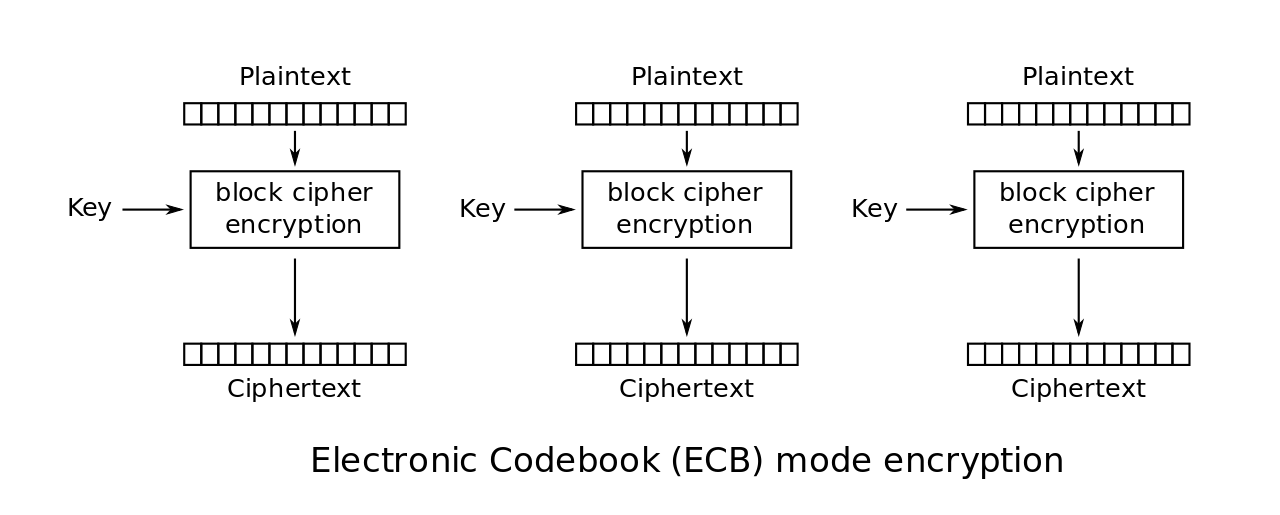
\includegraphics[scale = 0.25]{data/figures/ECB_encryption.png}
\caption{ECB: Every block of plaintext is simply encrypted with a key.}
\end{figure}

\begin{figure}
\centering
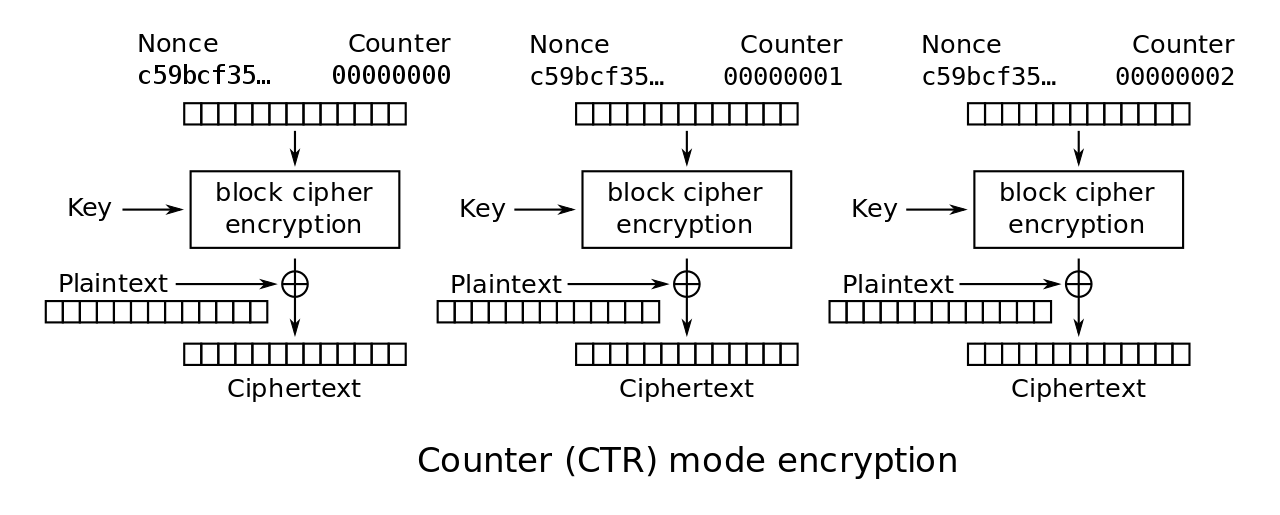
\includegraphics[scale = 0.25]{data/figures/CTR_encryption.png}
\caption{CTR: Every block of plaintext is XORed with a combination of initialization vector (here: Nonce) and counter, encrypted by the key to form the ciphertext.}
\end{figure}

In order for Electronic Codebook Mode to work correctly the bye array
containing the plaintext has to be padded though, as only byte arrays
with length l can be processed where l modulo 16 equals 0. Padding can
be implemented in multiple ways, this implementation does it as follows:

\begin{lstlisting}
def pad_input(ba):
    """pads bytearray to have a length % 16 = 0"""
    topad = 16 - len(ba) % 16
    if topad == 0:
        topad = 16 #ensures that last byte is always padding
    padding = bytearray([topad] * topad) # PKCS 5, 7
    return ba + padding
\end{lstlisting}

First it decides how many bytes the passed array is missing until the
length l of the array fulfills the requirement l modulo 16 equals 0. The
number of missing elements m is then appended m times to the array in
need of padding. If no padding is required a whole block gets padded.
This ensures the last byte of the decrypted string always contains the
information on how many bytes are padded and need to be removed, since
without this procedure a value for the last byte of one would be
ambiguous: does the last byte need to be removed since it is padding of
one or is it part of the message? This follows the concept of \cite[ch. 10.3 Note 2]{RFC2315}.

\begin{quote}
The array containing the plaintext is 357 bytes long. Since 357 modulo 16 = 5,
five bytes need to be added to the plaintext array. The present
implementation then adds an array containing the values \{5, 5, 5, 5,
5\} to the array.
\end{quote}

\hypertarget{implementation-6}{%
\subsubsection{Implementation}\label{implementation-6}}

\begin{lstlisting}
/*
 * Initializes the constant tables sbox, galois-field-multiplication-lookup and keys.
 * Performs AES-encryption on multiple, consecutive blocks.
 */
void encryptAES(uint8_t * restrict bytes, uint8_t * restrict initval,
                   const size_t bytecount, const uint8_t rounds)
{
        uint8_t sbox[256];
        uint8_t gal_mult_lookup[3][256];
        for(size_t i = 0; i < 256; i++) {
                sbox[i] = *initval++;
        }
        for(size_t i = 0; i < 3; i++) {
                for(size_t j = 0; j < 256; j++) {
                gal_mult_lookup[i][j] = *initval++;
                }
        }

        const uint8_t *keys = initval;
        uint8_t tempblock[16];

        for(size_t i = 0; i < bytecount; i += 16) {
                encryptBlock(&bytes[i], tempblock, keys,
                             rounds, sbox, gal_mult_lookup);
        }
}
\end{lstlisting}

The function takes four arguments. The first one is a restricted pointer
to an array containing the bytes that need to be encrypted. The second
argument is a restricted pointer to an array containing the
initialization values: first the elements of the S-box, followed by the
bytes of the GFMLT, while the rest are the bytes of the round keys. The
third is a constant unsigned variable which width equals the wordwidth
of the CPU architecture the source code gets compiled on. The last
argument is a constant byte containing the number of rounds. The
function starts by allocation an array of 256 unsigned bytes called
`sbox'. After that another array named `gal\_mult\_lookup' is allocated,
but this time it is two-dimensional, using three times 256 unsigned
bytes. The name is derived from `\textbf{Gal}ois field
\textbf{mult}iplication \textbf{lookup}table'. Both are initalized with
the three following for-loops. The first loop reads the first 256 bytes
from `initvar' and assigns them to `sbox'. The following two nested
for-loops iterate through the two dimensions of `gal\_mult\_lookup' and
assign the results of the Galois field multiplications in $GF(2^{8})$ to the
respective dimensions of the array.

After populating the arrays the pointer has moved far enough through
`initvals' that it now points to the first byte of the first round key.
To make this more clear and to enable possible compiler optimizations we
create a new pointer named `keys' pointing to a constant array, which is
in this case `initvals'. All future accesses to this array will be
through `keys' or descendants of this pointer. The last step before
starting the encryption routine is the creation of an array of sixteen
unsigned bytes called `tempblock'. The next for loop starts the
encryption. Every iteration processes one block and increments the loop
index variable by sixteen, so that it can point to the next block to be
processed. In every iteration of this loop the function `enrcryptBlock'
is called with the address of the current block to encrypt, a pointer to
the temporary block, a pointer to the array containing the round keys, a
variable containing the number of rounds, a pointer to the S-box and a
pointer to the GFMLT.

Since parallelisation of the de- and encryption routine seems to be a
worthwhile endeavour for the future, this function was already designed
with that in mind. An allocation of the temporary block as a local
variable instead of a global one avoids the need for thread
synchronization, since every thread would use their own temporary block,
if every thread spawned would use this function as a starting point.
